\subsection{Design}

\subsubsection{Microscope}

The starting point of the project was an Olympus BX60M fluorescence microscope. The BX60M is built for reflection microscopy, and includes a housing for brightfield and darkfield mirrors. For the new instrument, we added a mirror cube housing between the brightfield/darkfield mirror housing and the observation tube. This additional component housed a dichroic mirror, which enabled us to couple an external light source into the instrument and filter that light out of the path through the observation tube.

\begin{figure}[H]
    \centering
    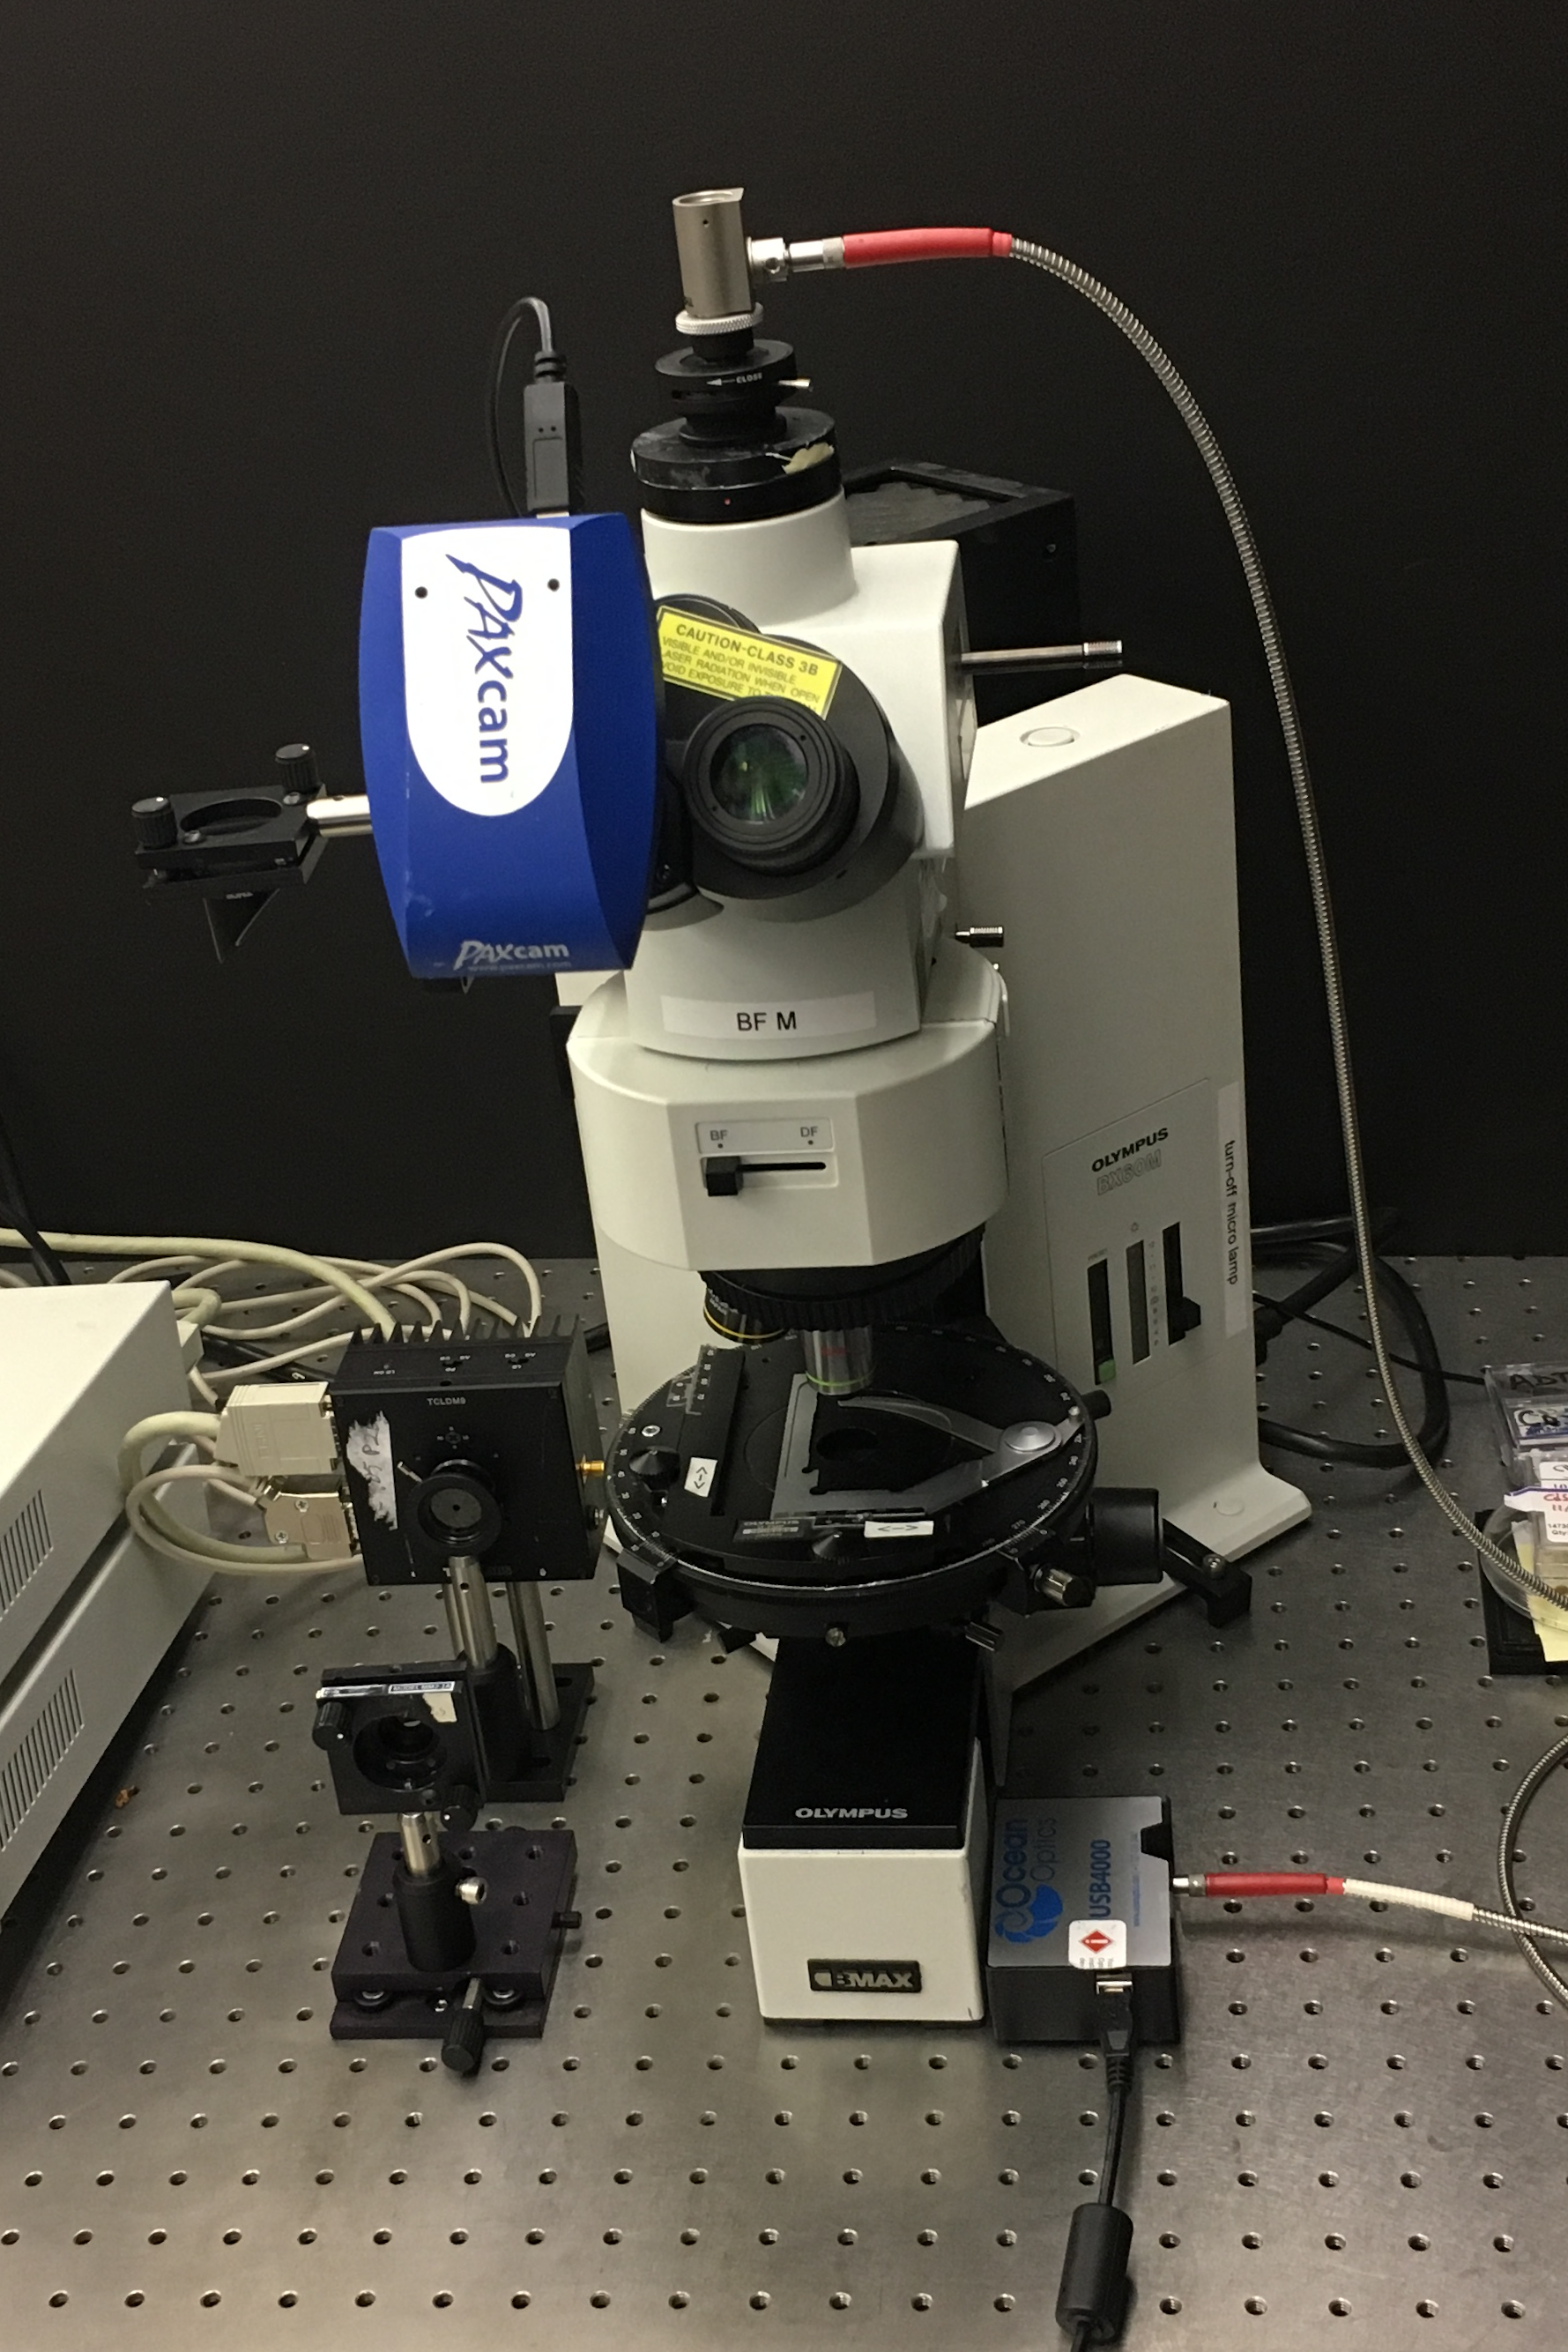
\includegraphics[width=0.5\textwidth]{img/microscope.png}
    \caption[Front view of microspectrometer instrument.]{Front view of microspectrometer instrument (laser controllers not pictured) built around Olympus BX60M fluorescence microscope. The laser diode mount and mirrors are shown on the left. Digital camera for sample imaging is mounted to the microscope eyepiece. At the top of the microscope's optical path we have mounted a collimating mirror, which collects filtered emissions and directs them into a USB spectrometer via a fiber optic.}
    \label{img:microscope}
\end{figure}


\subsubsection{Laser Excitation}
The BX60M is equipped with a xenon arc lamp, which is used for general observations under white light illumination. In order to measure photoluminescence, we require the use of a (mostly) monochromatic light source which is energetic enough to excite electrons in the sample.

\begin{figure}[h]
    \centering
    \includegraphics[width=.75\textwidth]{img/optical-diagram.png}
    \caption{Schematic diagram of the microspectrometer instrument.}
    \label{img:optical-diagram}
\end{figure}

Our instrument uses a diode laser as its light source. Specifically, we used a ThorLabs L405P20 laser diode (405 nm), TCLDM9 thermoelectrically-cooled mount, LDC 202 laser diode controller, and TED 200 temperature controller. To couple the laser and microscope, we used a set of two mirrors in a vertical beam fold configuration. This allowed for precise alignment of the laser to the optical axis of the microscope, which allows for maximal transmission of excitation light through the objective lens and onto the sample stage.

The laser diode housing and first mirror were mounted to an optical table. The laser starts parallel to the surface of the table, and the first mirror directs the beam upward. The second mirror in the beam fold was mounted to the end of a tube that extends out the side of the mirror cube housing. This mirror directs the vertical beam horizontally into the mirror. It seems preferable to mount both mirrors to the optical table for stability, but we were successful with this method by mounting the microscope to the table so that it and the second mirror did not move relative to the laser beam during normal operation.

\begin{figure}[H]
    \centering
    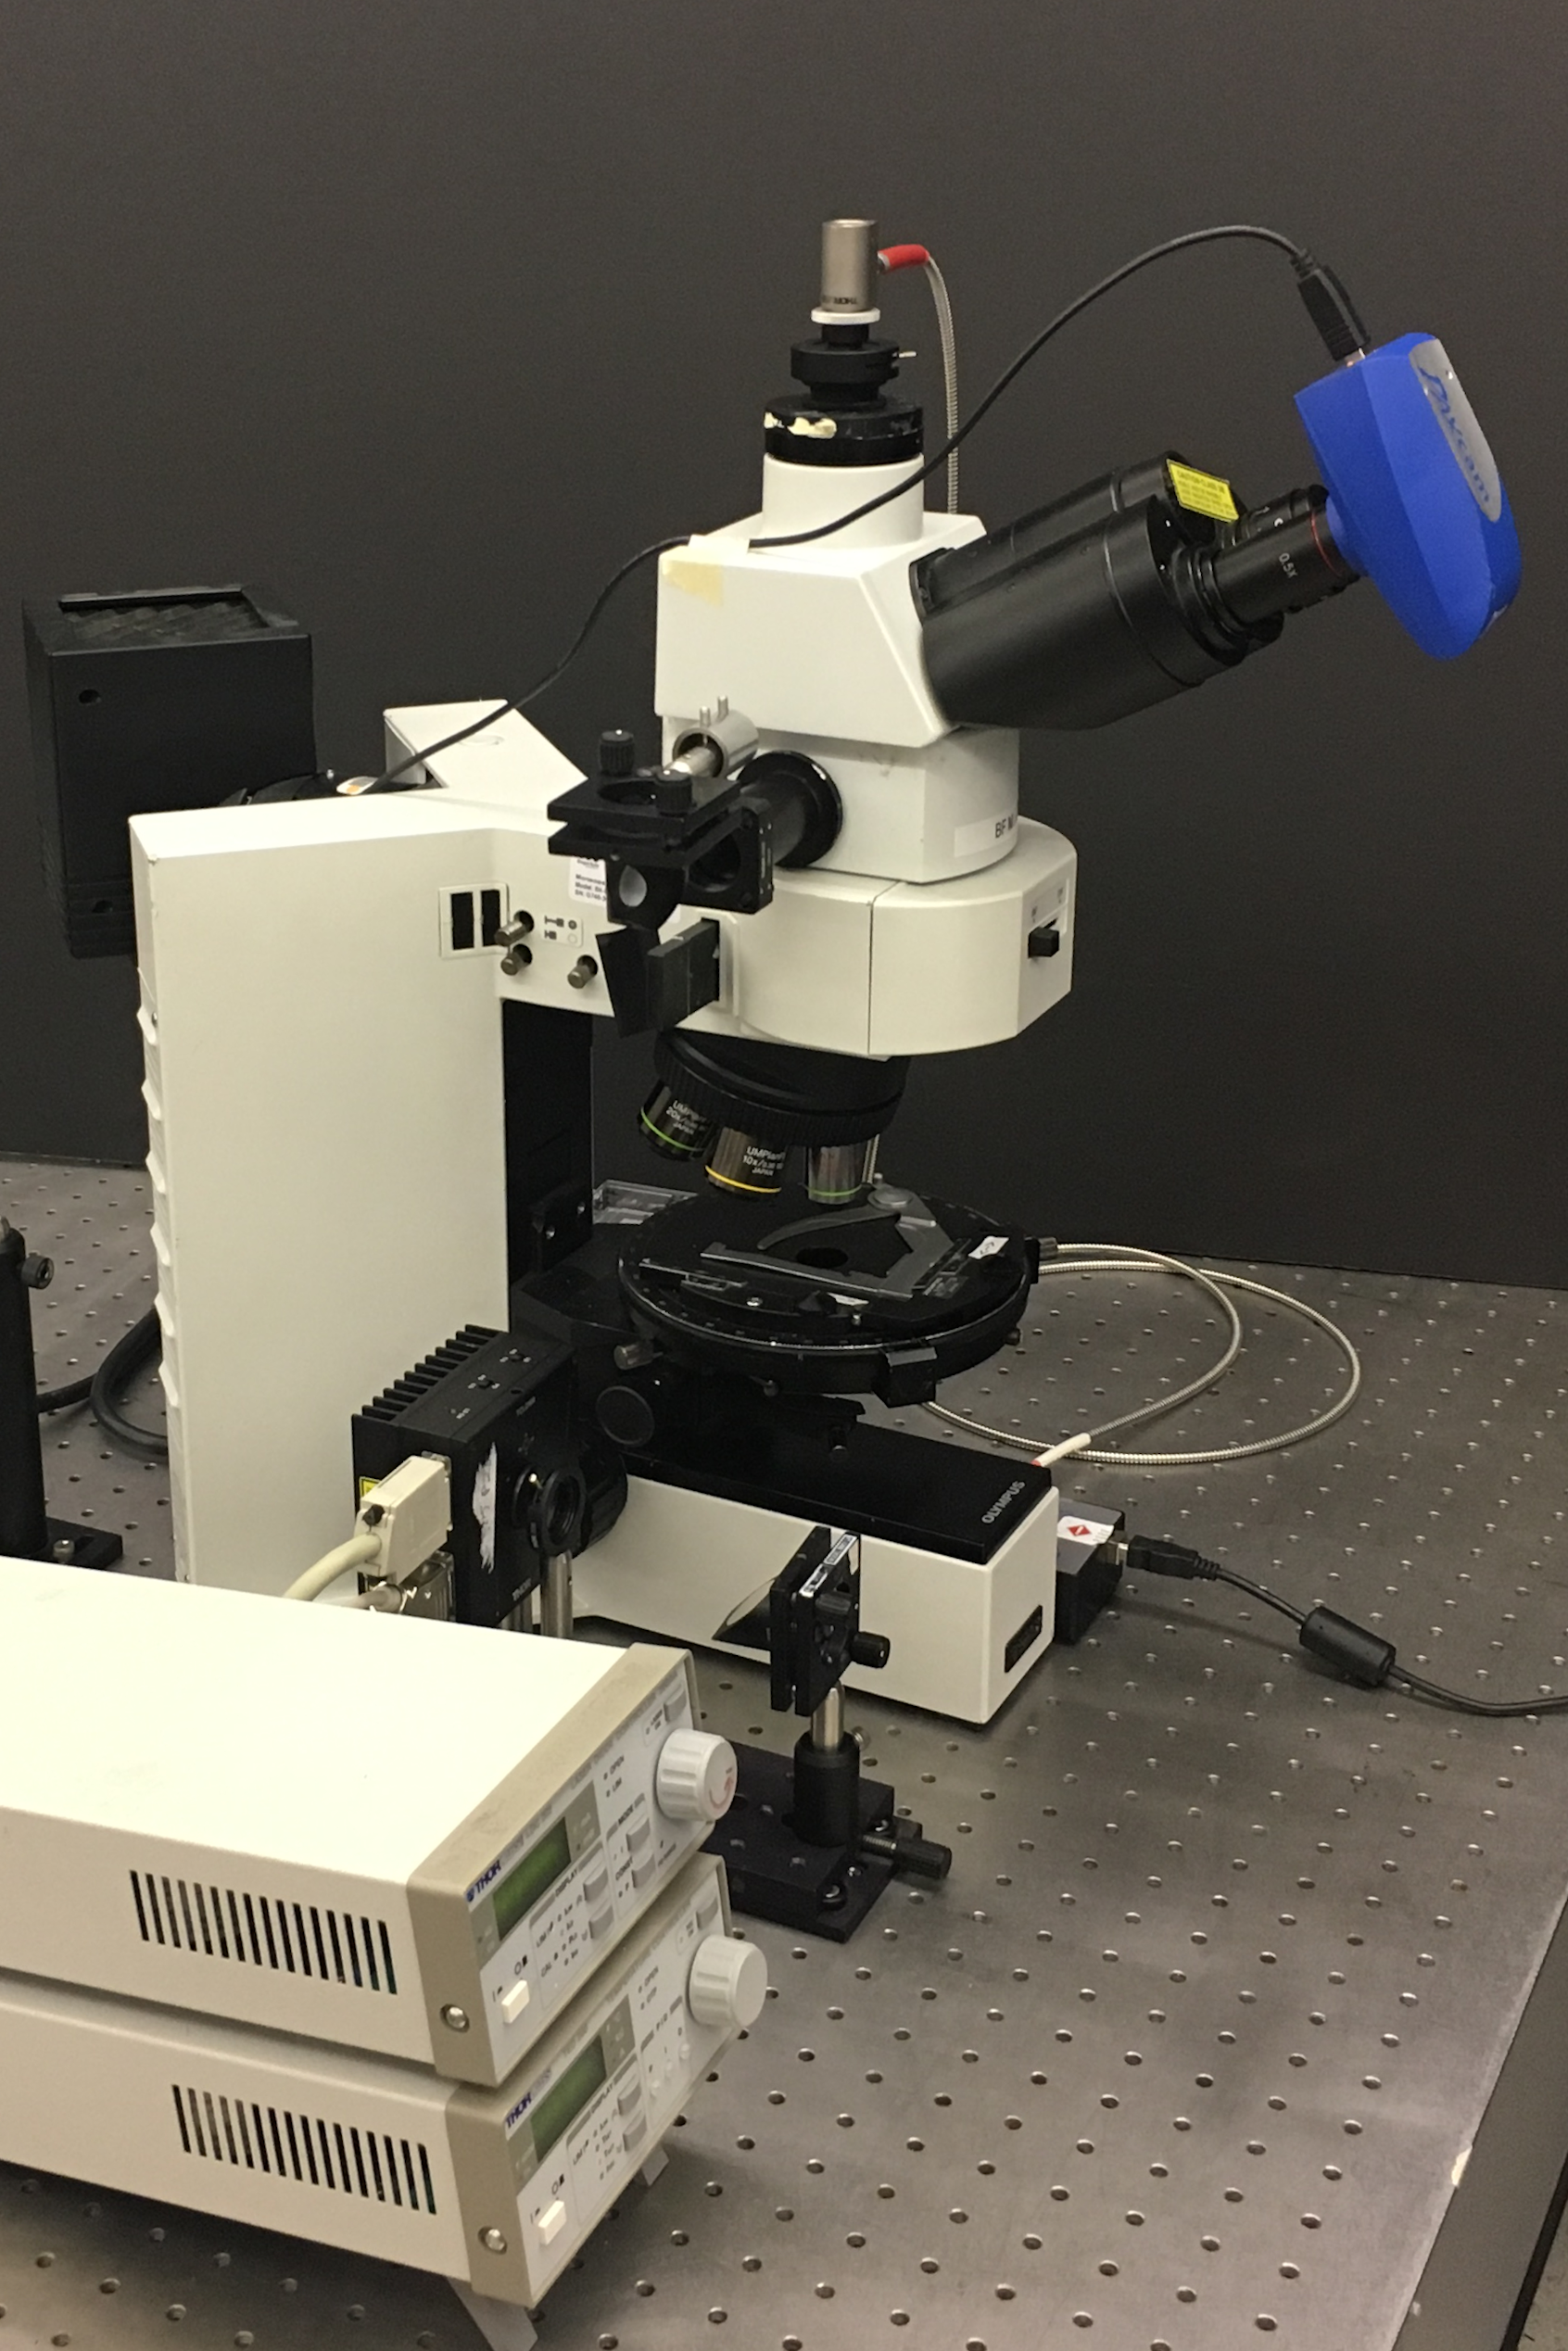
\includegraphics[width=0.5\textwidth]{img/microscope-side.png}
    \caption[Side view of microspectrometer instrument.]{Side view of microspectrometer instrument. Laser controllers are shown in the foreground. Between the controllers and the microscope, two flat mirrors and a dichroic mirror (not visible here) couple the laser light into the microscope's optical path.}
    \label{img:microscope-side}
\end{figure}

Due to limited space on the optical table, it was not feasible to align the laser diode housing and mirror cube housing in the plane of the table. To overcome this, our beam fold configuration also turns the beam 90 degrees in the plane of the table. The configuration we used has the laser beam initially pointed in the direction of the operator, then directed upward by the first mirror, then directed into the side of the mirror cube housing. While in operation, but particularly during laser alignment, precautions must be taken to protect the operator's eyes from direct exposure to the laser beam. The optical power of the laser is low enough that laser safety glasses (with high optical density near 405 nm) are sufficient, but beam blocks on the table may also be desireable in some cases.

We used a longpass dichroic mirror with a cutoff wavelength slightly higher than the excitation wavelength at 405 nm. This causes nearly all of the excitation light to be reflected in the direction of the sample. Because fluorescence will nearly always have a longer wavelength than the exciting photons, we expect the mirror to pass most of the light emitted by the sample and block any reflected excitation light.

\todo{Trinoc and fiber coupling} The microscope is equipped with a trinocular optic


\subsubsection{Measuring Spectra}
\todo{About the Ocean Optics?}

\begin{figure}[H]
    \centering
    \includegraphics[width=0.75\textwidth]{img/objective-sample.JPG}
    \caption[Sample on stage under laser illumination.]{A sample of CdSe quantum dots under laser illumination at 405 nm. Some of the violet laser light is reflected by the sample, but is difficult to distinguish from the sample's intense green emission.}
    \label{img:objective-sample}
\end{figure}


\subsubsection{Imaging}
\todo{About the camera}


\subsection{Laser Alignment}
We aligned the laser to the microscope's optical axis by iteratively adjusting the two flat mirrors that direct the beam into the side of the microscope. First, we adjust the position of the beam as it enters the mirror cube housing by moving the first mirror. A reticle made of photoluminescent laser viewing material was a particularly useful target when fixed to the opening on the side of the mirror cube housing. 

We then adjust the second mirror in the beam fold to change the angle at which the beam is incident on the dichroic mirror. This translates the beam across the back of the microscope nosepiece, where our target is the optical axis of the objective lens. In place of a lens, we fix an iris diaphragm to the nosepiece. We adjust the second mirror to position the laser in the center of the mostly-closed iris, which marks the location of the optical axis of a lens. This process is repeated until the laser spot is centered on both targets.

\subsection{Laser Controls}
\todo{About laser operation?}

\subsection{Imaging and Measuring Fluorescence}
\todo{About selecting an ROI, turning on the laser, taking pictures and measuring spectra}
